\section{Расчет параметров проектируемого изделия}

\subsection{Расчет теплового режима (выбор способа охлаждения;
  описание тепловых моделей;  оценка теплового режима). }

% Будет приведены аргументы в пользу выбора пассивного охлаждения в
% данном изделии, касающиеся простоты изделия и отсутствия каких-либо
% устройств выделяющих большой объём теплоты.

% Приведены расчёты соответствующие пассивному охлаждению в герметичном
% корпусе и в перфорированном корпусе.

В процессе эксплуатации РЭС на их элементы воздействуют температуры,
источниками которых выступают не только окружающая среда, но и сама
работающая техника. Любой блок РЭС с точки зрения теплофизики
представляет собой систему множества тел, в которых тепловая энергия
распределена в пространстве конкретного блока сложным
образом. Тепловую энергию выделяют активные элементы схемы за счет
потребления электрической энергии. Внутреннее тепловыделение,
совмещенное с воздействием температуры окружающей среды, приводит к
изменению электрических характеристик РЭС. Эти изменения могут быть
как обратимыми, так и необратимыми, а их величина варьируется от
незначительных до критических, способных вызвать отказ устройства.

Тепловой режим радиоэлемента определяется его температурным
состоянием, то есть пространственно-временным распределением
температуры внутри элемента. Существенные отклонения температуры
устройства от номинального значения, особенно в сторону повышения,
резко снижают его надежность из-за перегрева. Расчет теплового режима
проводится для сравнения полученных температурных характеристик с
предельно допустимыми температурами, на которые рассчитаны компоненты
РЭС, чтобы избежать превышения допустимых значений.

% Данные для расчёта

Из исходных данных был сделан вывод, что расчет теплового режима
должен подразумевать использование РЭС в герметичном корпусе.

Расчёт теплового режима для РЭС выполняется в указанном порядке
~\cite{Rotkop1976}:
\begin{enumerate}
\item Рассчитывается поверхность корпуса блока
  \begin{equation}
    S_{К} = 2 \cdot (l_1 l_2 + (l_1+ l_2)l_3) % (4.46)
  \end{equation}

  $$S_{К} = 2 \cdot (90 \cdot 80 + (90 + 80) \cdot 30) = 24600 мм² = 0.0123 м²$$
  
\item Определяется условная поверхность нагретой зоны:
  \begin{equation}
    S_{з} = 2 (l_1 l_2 + (l_1 + l_2) K_{з} l_3 ) % (4.39)
  \end{equation}

  $$S_{К} = 2 \cdot (90 \cdot 80 + (90 + 80) \cdot 30 \cdot 0,8) = 11280 мм² = 0.01128м²$$
\item Определяется удельная мощность корпуса блока:
%
\begin{equation}
  q_к = \frac{P_з}{S_к} % (4.45)
\end{equation}
%
$$ q_к = \frac{3,75}{0,0123} \sim 305 Вт/м² $$

\item Рассчитывается удельная мощность нагретой зоны:
 % 
  \begin{equation}
      q_з = \frac{P_з}{S_3} % (4.38)
    \end{equation}

$$ q_з = \frac{3,75}{0,0113} \sim 332 Вт/м² $$
\item По графику из пособия ~\cite{Rotkop1976}. Находится коэффициент
$\vartheta_1$ в зависимости от удельной мощности корпуса блока:
 %   
\begin{figure}[H]
  \centering
  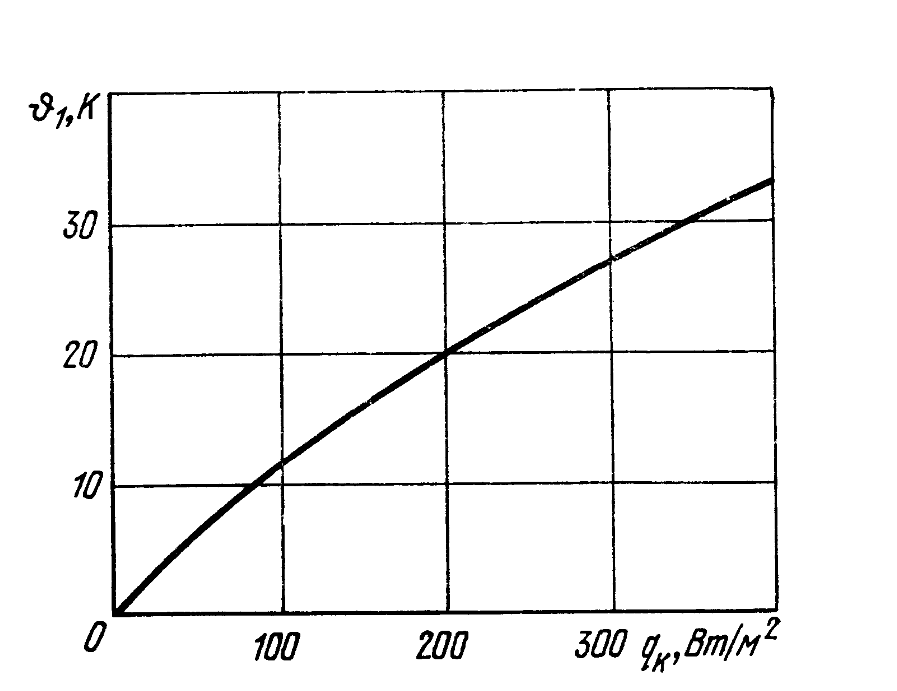
\includegraphics[scale=0.7]{Rotkop/Pic-4-6.png}
  \caption{Зависимость перегрева корпуса от удельной мощности}
\end{figure}

$$\vartheta_1 = 27  $$
\item По графику из пособия ~\cite{Rotkop1976}. Находится коэффициент
$\vartheta_2$ в зависимости от удельной мощности нагретой среды:

\begin{figure}[H]
  \centering
  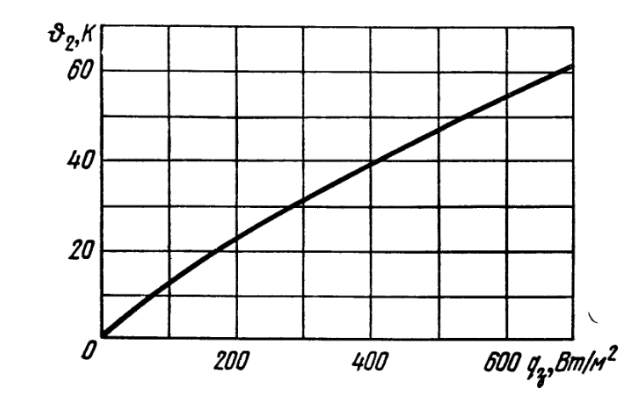
\includegraphics[scale=0.5]{Rotkop/Pic-4-4.png}
  \caption{Зависимость перегрева нагретой зоны от удельной мощности рассеивания}
\end{figure}

$$\vartheta_2 = 33  $$ 

\item Коэффициент $K_{Н1}$ в зависимости от давления среды вне корпуса
блока. Значение давления берётся из ГОСТ~\cite{GOST-15150-69}.

\begin{figure}[H]
  \centering
  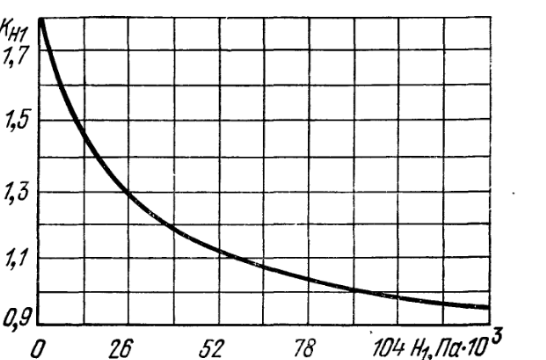
\includegraphics[scale=0.5]{Rotkop/Pic-4-7-b.png}
  \caption{Зависимость  $K_{Н1}$ от давления окружающей среды}
\end{figure}
$$K_{Н1}= 1,0$$

\item Коэффициент $K_{Н2}$ в зависимости от давления
  среды внутри корпуса блока.
  Значение берётся из ГОСТ~\cite{GOST-15150-69}.

  \begin{figure}[H]
  \centering
  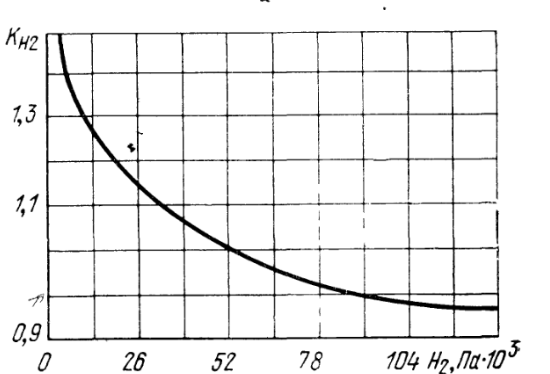
\includegraphics[scale=0.5]{Rotkop/Pic-4-8-b.png}
  \caption{Зависимость  $K_{Н2}$ от давления среды внутри аппарата}
\end{figure}
$$K_{Н2}= 1,0$$

\item Определяется перегрев корпуса блока:
  \begin{equation}
    \vartheta_к = \vartheta_1 \cdot K_{Н1}
  \end{equation}

  $$\vartheta_к = 27 \cdot 1 = 27 К$$
\item Рассчитывается перегрев нагретой зоны:
%
\begin{equation}
  \vartheta_з = \vartheta_к + (\vartheta_2 - \vartheta_1) \cdot K_{H2}
\end{equation}

$$\vartheta_з = 27 + (33 - 27) \cdot 1 = 33$$

\item Определяется средний перегрев воздуха в блоке:
%
\begin{equation}
  \vartheta_в = 0,5 \cdot (\vartheta_к + \vartheta_з)
\end{equation}

$$\vartheta_в = 0,5 \cdot (27 + 33) = 30К$$
\item Определяется удельная мощность элемента:
  \begin{equation}
    q_{эл} = \frac{P_{эл}}{S_{эл}}
  \end{equation}

  $$q_{эл}=\frac{0,25}{13,8 \cdot 10^{-3}} \sim 181 Вт/м²$$

\item Рассчитывается перегрев поверхности элементов:
  \begin{equation}
    \vartheta_{эл} = \vartheta_{з}\left(0,75 + 0,25 \cdot \frac{q_{эл}}{q_{з}}\right)
  \end{equation}

  $$\vartheta_{эл} = \vartheta_{з}\left(0,75 + 0,25 \cdot \frac{181}{332}\right) ~ 29К$$

\item Рассчитывается перегрев окружающей элементы среды:
  \begin{equation}
    \vartheta_{эл} = \vartheta_{к}\left(0,75 + 0,25 \cdot \frac{q_{эл}}{q_{з}}\right)
  \end{equation}

  $$\vartheta_{эл} = \vartheta_{к}\left(0,75 + 0,25 \cdot \frac{181}{332}\right) ~ 24К$$

\item Определяется температура корпуса блока:
  \begin{equation}
  T_к = \vartheta_к +  Tc
\end{equation}
$$  T_к = 27 + 313 = 340 К$$
\item Опредяеляется температура нагретой зоны:
  \begin{equation}
  T_з = \vartheta_з +  T_c
\end{equation}

$$T_з = 33 + 313 = 346 К$$
\item Находится температура поверхности элементов:  

\begin{equation}
  T_{эл} = \vartheta_{эл} + T_c
\end{equation}
$$T_{эл} = 30 + 313 = 343 К$$


\item Находится температура воздуха в блоке:
  \begin{equation}
  T_{в}   = \vartheta_{в} + T_c
\end{equation}
$$  T_{в}   = 30 + 313 = 343 К$$
\end{enumerate}

\subsection{Расчёт на механические воздействия. }

% По толщине, длине, ширине и массе печатной платы будет определена
% собственная частота печатной платы согласно ~\cite{Kalenkovich2012}
% года издания.

Под механической прочностью понимают способность констуркции РЭС и его
элементов противостоять механическим воздействиями без разрушения.

При расчете конструкции и ее элементов на механическую прочность
определяют уровни ее запасов.  Обычно отсуствие достаточной
механической прочсности вдеёт к появлению обрывов, трещин сколов,
срывов элементов со своих посадочных мест, к поломкам корпусов ЭРЭ,
смятию, значительным уровням остаточных деформаций, что ведет к
электрическому отказу конструкции РЭС.
При этом под отказом РЭС здесь понимается также и уход его
электрических параметров за допустимые пределы. Вместе с тем
электрический отказ РЭС может наступать в результате механических
воздействий за счет значительных уровней упругой деформации некоторых
констурктивных элементов даже при их достаточной механической
прочности. При таких деформациях могут происходить короткие замыканиях
между элементмаи, приводящие к электрическому пробою или к ухудшению
электрических параметров РЭС. Все это в соответвии с теорией
сопротивления материалов будет свидетелсьтвовать о недостаточной
жесткости элементов конструкции~\cite{Kalenkovich1989}.

Аналогичные явления в конструкциях будут наблюдаться при механических
воздействиях, когда такие конструктивы, как платы, будут испытыать
механическую нагрузку вдоль их продольной оси.
При достижении данной нагрузкой некоторого критического значения может
происходить продольный изгиб платы~\cite{Kalenkovich1989}.

Целью расчета является определение действующих на элементы изделия
перегрузок при наличии вибрации, а также максимальных перемещений.
При необходимости производится выбор и расчет системы
аммортизации~\cite{Kalenkovich2012}.

Исходные данные для расчета:
\begin{itemize}
\item длина ПП a - 90 мм,
  
\item ширина ПП b - 80 мм,
  
\item толщина печатной платы ПП h - 1,5 мм,
  
\item масса печатной платы с ЭРЭ m - 186.1г.
\end{itemize}

Определяем частоту собственных колебаний печатной платы, как
частоту собственных колебаний, равномерно нагруженной пластины по
формуле ~\cite{Kalenkovich2012}:
\begin{equation}
  f_0 = \frac{1}{2\pi}\frac{K_{\text{б}}}{a^2}\sqrt{\frac{D}{M}ab}
\end{equation}
Где:
\begin{itemize}
\item $a$ и $b$ - длина и ширина пластины;

\item $D$ - цилиндрическая жесткость;
\item $M$ - масса пластины с элементами.
\item $K_{\alpha}$ - коэффициент, зависящий от способа закрепления сторон пластины.
\end{itemize}

Характеристика стеклотекстолита приведена в таблице 5.1.

\begin{table}[H]
  \caption{Характеристики стеклотекстолита}
  \centering
  \begin{tabular}{|p{0.25\linewidth} | p{0.35\linewidth}| p{0.2\linewidth} |}
    \hline
    Материал & Модуль упругости, $E \times 10^{10},$ Н/м²& Коэффициент Пуассона, $\gamma$ \\
    \hline
    Cтетклотекстолит & 3,2 & 0,279 \\
    \hline
  \end{tabular}
\end{table}

\subsection{Расчет конструктивно-технологических параметров печатных плат. }

% Основываясь на~\cite{Kostukevich2012}, приведен расчёт
% объёмно-компоновочных характеристик устройства на основе данных о
% имеющихся на ней компонентах и коэффициенте заполнения.
Под компоновкой электронной аппаратуры понимается процесс размещения
комплектующих модулей, изделий электронной техники (ИЭТ) и деталей ЭА
на плоскости или в пространстве с определением основных геометрических
форм и размеров, а также ориентировочное определение массы изделия.
На практике задача компоновки чаще всего решается путем размещения
готовых элементов с заданными формами, размером и весом на плоскости с
учетом электрических, магнитных, механических, тепловых и других видов
связи. При компоновке нужно стремиться к тому, чтобы ~\cite{Kostukevich2012}:
\begin{enumerate}
\item обеспечивалось отсутствие заметных паразитных электрических и магнитных взаимосвязей,
  влияющих на технические характеристики изделия;
  
\item взаимное расположение элементов обеспечивало технологичность сборки и монтажа,
  легкий доступ для контроля, ремонта и обслуживания;
  
\item изделие удовлетворяло требованиям технической эстетики;
\item габариты и масса изделия были минимальными.
\end{enumerate}

Существуют различные способы компоновки аппаратуры.
Необходимо выполнить аналитический расчет компоновочных параметров,
в основе которого лежит представление геометрических параметров ЭА
в виде чисел ~\cite{Kostukevich2012}.

Исходными данными для компоновочного расчета являются
~\cite{Kostukevich2012}:
\begin{itemize}
\item перечень элементов;  
\item габаритные и установочные размеры ИЭТ.
\end{itemize}

Методика расчёта заключается в следующем ~\cite{Kostukevich2012}:
\begin{enumerate}
\item Определяется суммарная площадь $S_{\text{ИЭТ}}$, занимаемая всеми ИЭТ:
  \begin{equation}
    S_{\text{ИЭТ}} = \sum^N_{i=1}S_{yi}
  \end{equation}
  где $S_{yi}$ - значение установочной площади \textit{i}-го элемента;
  \textit{n} —  количество элементов.
%
  $$ S_{\text{ИЭТ}}= 2851 \text{ мм²}$$
%
\item Рассчитывается приблизительная площадь печатной платы с учетом
  способа монтажа (односторонний, двусторонний):
  \begin{equation}
    S_{\text{Пл}} = \frac{S_{\text{ИЭТ}}}{(k_{\text{ЗПл}} \cdot m)}
  \end{equation}
  %
  где $k_{\text{ЗПл}}$ — коэффициент заполнения платы печатной, как правило,
  должен быть в пределах от 0,3 до 0,8;
  m — количество сторон монтажа (1,2).
  В данном случае количество сторон монтажа равно $m=1$.
  %
  $$S_{\text{Пл}} = 3563.75 \text{ мм²}$$
\end{enumerate}


Исходя из рассчитанной площади платы и высоты ИЭТ определить
приблизительные габаритные размеры~\cite{Kostukevich2012}.

При оценке приблизительных габаритных размеров всего устройства два
размера из трех определяют по рассчитанным размерам платы печатной с
учетом допусков на зазоры между платой и корпусом, толщины корпуса,
особенностей дизайна устройства и т. п.
Третий размер определяется с учетом максимально высоких элементов,
размещаемых на плате, и размеров, обусловленных особенностью
разрабатываемой конструкции (способ крепления платы в корпусе,
толщина корпуса, наличие дополнительных деталей на корпусе и т. п.) ~\cite{Kostukevich2012}.

Допускается выполнять предварительный расчет габаритных размеров
электронной аппаратуры по следующей методике ~\cite{Kostukevich2012}:
\begin{enumerate}
\item Определяется суммарный объем, занимаемый всеми ИЭТ и деталями:
  \begin{equation}
    V_{\textit{ИЭТ}} = \sum^N_{i=1}\vartheta_i +   \sum^M_{i=1}\vartheta_j
  \end{equation}
%
где $\vartheta_i$ - значение объёма \textit{i}-го ИЭТ;
$\vartheta_j$ — значение объёма \textit{j}-й детали;
\textit{N} — количество ИЭТ;
\textit{M} — количество деталей.
%
$$V_{\textit{ИЭТ}} =  2694 \text{мм}^3$$
\item Оценивается приблизительный объем всего устройства:
  \begin{equation}
    V_{\text{У}} = \frac{V_{\text{ИЭТ}}}{K_{\text{З}}}
  \end{equation}
%
  $$V_{\text{У}} =3367.5 \text{мм}^3$$
%
\end{enumerate}
%
Таким образом был рассчитан объём печатной платы на основе данных о
имеющихся на ней компонентах и коэффициенте заполнения.
Реальный же объём может отличаться, по той причине, что при таком
подсчёте не было учтено место отведенное под дорожки между
компонентами.

\subsection{Расчёт электромагнитной совместимости}

% Согласно одному из актуальных пособий будет выбрана методика расчёта
% электромагнитной совместимости о осуществлён расчёт на основании этой
% методики.

\subsection{Полный расчёт надёжности. }

Под надёжностью понимают свойство изделия сохранять в течение
заданного времени в пределах установленных норм значения
функциональных параметров при определённых условиях (заданные режимы и
условия эксплуатации, техническокого обслуживания, хранения и
транспортирования)~\cite{Borovikov2010}.

В теории и практике надёжности технических изделий широко используют
понятие наработка, под которой понимают продолжительность работы
изделия, выраженную в часах, циклах переключения или других единиц в
зависимости от вида и функционального назначения изделия ~\cite{Borovikov2010}.

Под отказом понимают полную или частичную потерю изделием
работоспособности вследствие ухода одного или нескольких
функциональных параметров за пределы установленных норм, указанных в
технической документации~\cite{Borovikov2010}.

Проведём уточнённый расчёт показателей безотказности функционального модуля:
\begin{enumerate}
\item Находим коэффициент электрической нагрузки элементов, пользуюясь
картами электрических режимо и эксплуатационными электрическими
характеристиками используемыми в модуле.

Коэффициент электрической нагрузки элементов равен
\begin{equation}
  K_{\text{Н}} = \frac{F_{\text{раб}}}{F_{\text{ном}}}
\end{equation}

% При этом исходя из того, что в данной работе расчёт производится на
% раннем этапе проектирования, выходит возможным, на
% основании данных полученных в результате САПР для симуляции
% электронных схем, узнать показатели $F_{\text{раб}}$ и
% на основании полученных данных подбирать компоненты из широкого
% ассортимента представленных на рынке с таким показателем
% $F_{\text{ном}}$ чтобы искуственно изменять коэффицент
% $  K_{\text{Н}}$ в лучшую сторону.


Симуляция схемы не была произведена, по той причине, что на момент
написания работы не была готова прошивка для микроконтроллера в схеме,
однако, приняв во внимание,  вышеописанную возможность примем
$K_{\text{Н}}$ у элементов равным $0,8$.
\item Определим максимальную температуру элементов модуля при его
  работу в составе РЭУ.
  Для учета влияния температуры на эксплуатационную интенсивность
  отказов элементов  $\lambda_{\text{Э}}$ принято во внимание
  верхнее значение предельной рабочей температы
  ($t_{\text{раб.max}}= 40°C$), cоответствующей РЭУ
  исполнения УХЛ4.2 по ГОСТ 15150-69, и возможное увеличение предельной рабочей температуры на значение
  $\Delta t_C = 10°C$ за счёт нагрева РЭУ и, следовательно модуля в составе РЭУ.
  Предельная рабоачая температура $t_{эл.max}$ теплонагруженных
  элементов (ИМС, транзисторы, диоды, мощные резисторы) определена как \cite{Borovikov2010}:
  \begin{equation}
    t_{\text{эл.max}} = (t_{\text{раб.max}} + \Delta t_C) + \Delta t_{\text{з}} = (40 + 10) +15 = 65°С
  \end{equation}
  где $\Delta t_{\text{з}}$ — перегрев нагретой зоне конструкции РЭУ
  Нагретая зона — это гиптотетический объём, в котором условно
  рассеивается вся тепловая энергия, выделяемая РЭУ.

  Значение величины $t_{эл.max}$  для нетеплонагруженных элементов
  (конденсаторы, слабонагруженные резисторы, соединительс, кварцевый резонатор)
  подсчитано как ~\cite{Borovikov2010}:
  \begin{equation}
    t_{\text{эл.max}} = (t_{\text{раб.max}} + \Delta t_C) + \Delta t_{\text{з}} = (40 + 10) +10 = 60°С
  \end{equation}
%
\item Пользуясь таблице 5.3 из источника~\cite{Borovikov2010} находим
  справочные значения интенсивности отказов элементов модуля.

\item По таблице 5.1 из ~\cite{Borovikov2010} выбираем математические
модели расчёта эксплуатационной интеcивности отказов элементов
$\lambda_{\text{Э}}$
% ---

\item Определяем значения поправочных коэффициентов, входящих в
выбранные модели расчёта эксплутационной интесивности отказов
элементов $\lambda_{\text{Э}}$
\item Для каждого элемента находим произведение поправочных
коэффициентов, и значение эксплуатационной интесивности отказов
$\lambda_{\text{Э}}$.

\begin{sidewaystable}
  \centering
  \small
  \caption{Расчёт эксплуатационной безоткзоности элементов модуля}
  \begin{tabular}{|l |l |l |l |l |l |l |l |l |l |l |l |l |l |l |l |l |l |}
    \hline
Designator  &   λБ  & λe                 & Кис & Кр & Кt & Ккорп & Кv & Кф & Кд & Кu & Кс & Kr & Км & Кк & Кэ & Кп & λe   \\ \hline
R1...R4     & 0,044 & λб Kр Kr Км Kэ Kп  & 1 & 0,34 & 1 & 1 & 1 & 1 & 1 & 1 & 1 & 0,7 & 0,7 & 1 & 1 & 1 & 0,1615 \\ \hline
R5...R8     & 0,183 & λб Kр Kr Км Kэ Kп  & 1 & 0,99 & 1 & 1 & 1 & 1 & 1 & 1 & 1 & 0,9 & 0,7 & 1 & 1 & 1 & 0,6209 \\ \hline
R9...R10    & 0,044 & λб Kр Kr Км Kэ Kп  & 1 & 0,34 & 1 & 1 & 1 & 1 & 1 & 1 & 1 & 0,7 & 0,7 & 1 & 1 & 1 & 0,1615 \\ \hline
R13         & 0,044 & λб Kр Kr Км Kэ Kп  & 1 & 0,34 & 1 & 1 & 1 & 1 & 1 & 1 & 1 & 1 & 0,7 & 1 & 1 & 1 & 0,2395  \\ \hline
R14         & 0,044 & λб Kр Kr Км Kэ Kп  & 1 & 0,34 & 1 & 1 & 1 & 1 & 1 & 1 & 1 & 0,7 & 0,7 & 1 & 1 & 1 & 0,16 \\ \hline
R15         & 0,044 & λб Kр Kr Км Kэ Kп  & 1 & 0,34 & 1 & 1 & 1 & 1 & 1 & 1 & 1 & 1 & 0,7 & 1 & 1 & 1 & 0,24  \\ \hline
C1          & 0,173 & λб Кр Кс Кэ Кп  & 1 & 0,7 & 1 & 1 & 1 & 1 & 1 & 1 & 0,5768 & 1 & 1 & 1 & 1 & 1 & 0,41 \\ \hline
C2          & 0,173 & λб Кр Кс Кэ Кп  & 1 & 0,7 & 1 & 1 & 1 & 1 & 1 & 1 & 0,3344 & 1 & 1 & 1 & 1 & 1 & 0,24 \\ \hline
C3          & 0,173 & λб Кр Кс Кэ Кп  & 1 & 0,7 & 1 & 1 & 1 & 1 & 1 & 1 & 0,2 & 1 & 1 & 1 & 1 & 1 & 0,14 \\ \hline
C4, C5      & 0,022 & λб Кр Кс Кэ Кп  & 1 & 0,7 & 1 & 1 & 1 & 1 & 1 & 1 & 0,1412 & 1 & 1 & 1 & 1 & 1 & 0,099 \\ \hline
DA1         & 0,028 & λб Кt Кис Ккорп Кv Кэ Кп & 0,96 & 1 & 1,3703 & 1 & 1 & 1 & 1 & 1 & 1 & 1 & 1 & 1 & 1 & 1 & 1,320 \\ \hline
DD1         & 0,023 & λб Кt Кис Ккорп Кv Кэ Кп & 0,75 & 1 & 1,412 & 1 & 1 & 1 & 1 & 1 & 1 & 1 & 1 & 1 & 1 & 1 & 1,054 \\ \hline
HA1         & 0,034 & λбКэКп & 1 & 1 & 1 & 1 & 1 & 1 & 1 & 1 & 1 & 1 & 1 & 1 & 1 & 1 & 1 \\ \hline
HL1         & 0,034 & λбКрКэКп & 1 & 0,04985 & 1 & 1 & 1 & 1 & 1 & 1 & 1 & 1 & 1 & 1 & 1 & 8 & 0,3988 \\ \hline
SA1         & 0,058 & Λб Кк Кf КрКэКп & 1 & 1,96 & 1 & 1 & 1 & 1 & 1 & 1 & 1 & 1 & 1 & 1 & 1 & 1 & 1,960 \\ \hline
SA2         & 0,058 & Λб Кк Кf КрКэКп & 1 & 1,96 & 1 & 1 & 1 & 1 & 1 & 1 & 1 & 1 & 1 & 1 & 1 & 1 & 1,960 \\ \hline
VD1         & 0,091 & λб Кр Кф Кд Кu Кэ Кп    & 1 & 0,05 & 1 & 1 & 1 & 1,5 & 0,6 & 0,8183 & 1 & 1 & 1 & 1 & 1 & 1 & 0,037 \\ \hline
VD2         & 0,091 & λб Кр Кф Кд Кu Кэ Кп    & 1 & 0,05 & 1 & 1 & 1 & 1,5 & 0,6 & 0,8183 & 1 & 1 & 1 & 1 & 1 & 1 & 0,037 \\ \hline
VD3         & 0,091 & λб Кр Кф Кд Кu Кэ Кп    & 1 & 0,05 & 1 & 1 & 1 & 1,5 & 0,6 & 0,8183 & 1 & 1 & 1 & 1 & 1 & 1 & 0,037 \\ \hline
VT1         & 0,044 & λб Кр Кф Кд Кu Кэ Кп    & 1 & 0,18 & 1 & 1 & 1 & 0,7 & 0,5 & 2,2831 & 1 & 1 & 1 & 1 & 1 & 1 & 0,14 \\ \hline
X1,X5       & 0,0104 & λб Кр Кк Кn Кэ Кп  & 1 & 0,5 & 1 & 1 & 1 & 1 & 1 & 1 & 1 & 1 & 1 & 2,86 & 1 & 8 & 11,49 \\ \hline
X2          & 0,0104 & λб Кр Кк Кn Кэ Кп  & 1 & 0,5 & 1 & 1 & 1 & 1 & 1 & 1 & 1 & 1 & 1 & 1,36 & 1 & 8 & 5,47 \\ \hline
X3          & 0,0104 & λб Кр Кк Кn Кэ Кп  & 1 & 0,5 & 1 & 1 & 1 & 1 & 1 & 1 & 1 & 1 & 1 & 2,02 & 1 & 8 & 8,11 \\ \hline
X4          & 0,0104 & λб Кр Кк Кn Кэ Кп  & 1 & 0,5 & 1 & 1 & 1 & 1 & 1 & 1 & 1 & 1 & 1 & 2,02 & 1 & 1 & 1,02 \\ \hline
ZQ1         & 0,026 & λб Кt Кэ Кп         & 1 & 1 & 1,29 & 1 & 1 & 1 & 1 & 1 & 1 & 1 & 1 & 1 & 1 & 1 & 1,29 \\ \hline
    
  \end{tabular}
\end{sidewaystable}


\item Подсчитываем эксплуатационную интенсивность отказов модуля.
  Просуммировав значения, приведенные в последнем столбце.
  $$\lambda_{\text{М}} = 36,53 \cdot 10^{-6} \text{1/ч}$$
  
\item Находим наработку на отказ:
  $$T_0 = 1 / \Lambda_{\text{М}} = 27,377 \text{часов}$$
\end{enumerate}

\newpage

%%% Local Variables:
%%% mode: LaTeX
%%% TeX-master: "main"
%%% LaTeX-biblatex-use-Biber: t
%%% End:
